\documentclass[a4paper,12pt]{article}
\usepackage[utf8]{inputenc}
\usepackage{amsmath}
\usepackage{graphicx}
\usepackage{geometry}
\usepackage{hyperref}
\geometry{a4paper, margin=1in}

\title{Evaluation von Photogrammetrie 3D-Scan für CFD-Simulationen}
\author{Peter Kuhn}
\date{2024-05-26}

\begin{document}

\maketitle

\tableofcontents

\section{Einleitung}\label{sec:Einleitung}
Das Ziel ist es zu bewerten, wie geeignet ein Photogrammetrie 3D-Scan für eine CFD-Simulation ist.

Die Vorteile eines photogrametrie 3d scanners im smartphone ist, dass smartphones sehr weit verbreitet sind. Die Frage ist wie gut dieser scanner geeignet ist.

Dazu wird eine Simulation mit 3D-gescannten Objekten und eine Simulation mit den Originaldimensionen des Objekts gemacht.

Als Untersuchungsobjekt wurde eine Kuh gewählt. In der theoretischen Physik ist es üblich, komplexe Formen zu vereinfachen, und eine Kuh wird oft als sphärisch angenommen. Ein bekanntes Meme aus dem Jahr 2015 verglich den Luftwiderstand einer Kuh mit dem eines Jeeps. Um dieses Konzept aufzugreifen, wird in dieser Arbeit der \( c_d \)-Wert (Luftwiderstandsbeiwert) einer 3D-gescannten Kuh bestimmt.
\newpage

\begin{figure}[h]
    \centering
    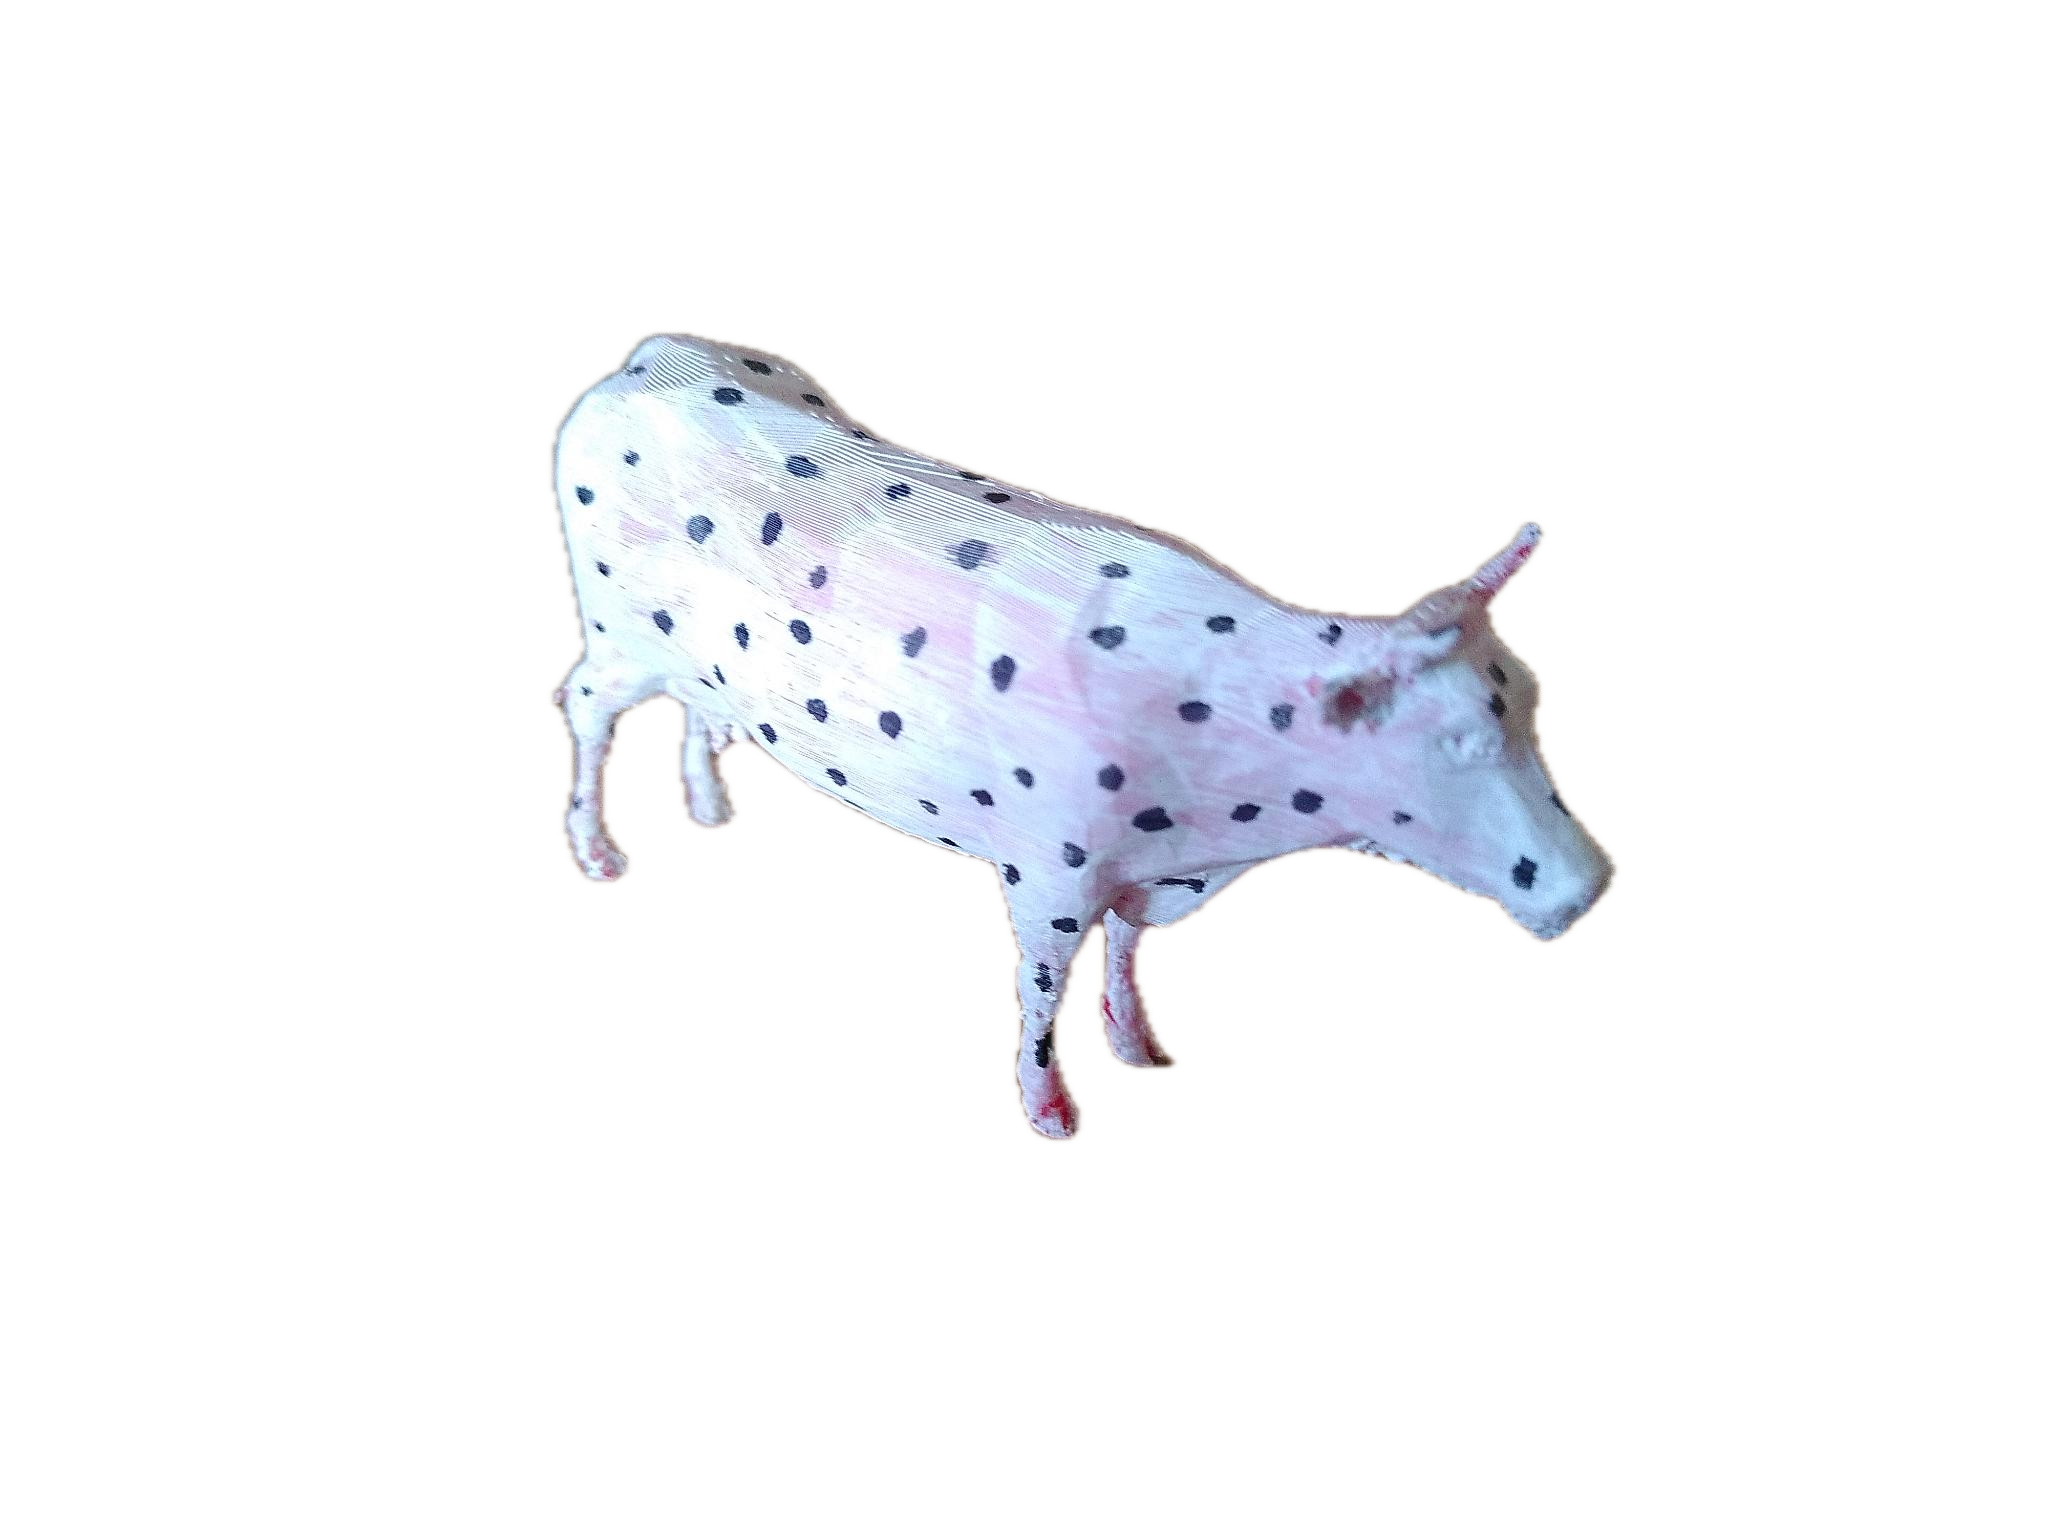
\includegraphics[width=0.5\textwidth]{signal-2024-05-26-124612.png}
    \caption{3D-gedruckte Kuh, angemalt}
    \label{fig:cowObj}
\end{figure}

Der Widerstandsbeiwert \( c_d \) ist definiert als

\begin{equation}
c_d = \frac{2 F_d}{\rho u^2 A}
\end{equation}

wobei:
\begin{itemize}
    \item \( F_d \) die Widerstandskraft ist, die per Definition die Kraftkomponente in Richtung der Strömungsgeschwindigkeit ist;
    \item \( \rho \) die Massendichte des Fluids ist;
    \item \( u \) die Strömungsgeschwindigkeit des Objekts relativ zum Fluid ist;
    \item \( A \) die Referenzfläche ist.
\end{itemize}

\section{Aufbau}

\subsection{Geometrie}
Um einen Vergleich der Geometrie zu machen, braucht es zwei Geometrien. Hierfür wurde zum einen eine frei verfügbare Low-Poly-Kuh und zum anderen der Scan des 3D-Drucks der Low-Poly-Kuh gemacht.

\begin{figure}[h]
    \centering
    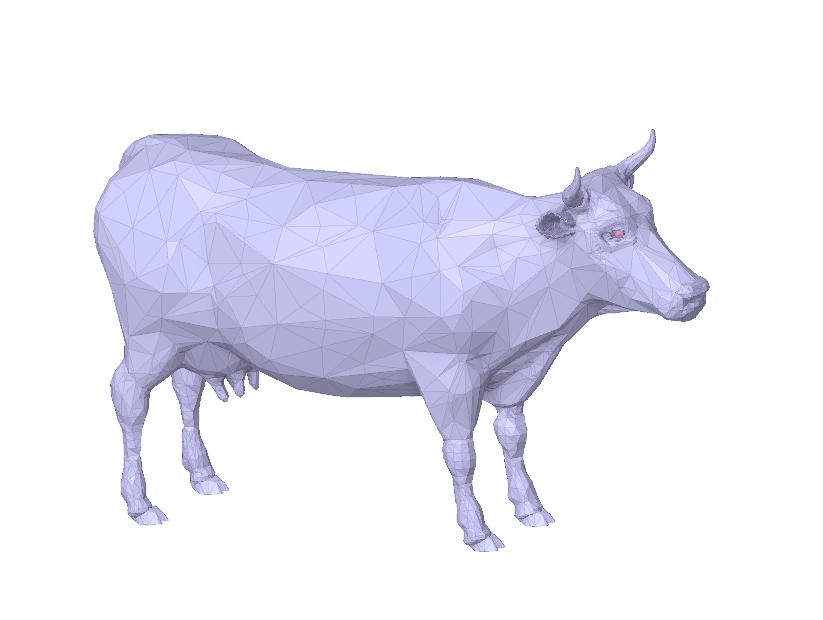
\includegraphics[width=0.5\textwidth]{cow.PNG}
    \caption{Original STL aus dem Internet}
    \label{fig:Orggeometry}
\end{figure}
\newpage
\subsection{3D-Scan Workflow}
Um die gescannte Geometrie zu erhalten, wurden verschiedene Techniken ausprobiert. Der folgende Ablauf hat sich als erfolgreich erwiesen:

\begin{enumerate}
\item Eine STL 3D-Datei einer Kuh im Internet finden \href{https://www.printables.com/de/model/175429-cow}{(Link zur Kuh-Datei)}
\item Mit Prusa Slicer die STL-Datei in G-Code umwandeln
\item Mit einem Ultimaker 2+ 3D-Drucker den G-Code in ein physisches Objekt umsetzen
\item Den 3D-Druck in Weiß und Schwarz anmalen, um Reflexionen zu vermeiden und Tracking-Punkte zu setzen
\item Mit einem Smartphone und externen LEDs unter Verwendung der Software Polyscan 130 Bilder aufnehmen und diese auf externen Servern in eine GLTF-Datei umwandeln und exportieren
\item Mit Blender die GLTF-Datei bearbeiten, den Boden entfernen und als STL-Datei exportieren
\item In ANSYS Spaceclaim mit der Funktion Shrinkwrap eine zusammenhängende STL-Datei erstellen
\item In nTop die STL-Datei in eine implizite Geometrie umwandeln
\item In nTop aus der impliziten Geometrie eine Konstruktion ableiten und als STEP-Datei exportieren
\item In NX die Konstruktion der Luft um die Kuh als prt-Datei (siehe Abbildung \ref{fig:nx}) erstellen und als STEP-Datei exportieren
\item In ANSYS die STEP-Datei importieren und normal vernetzen
\end{enumerate}

Dieser Prozess ist herausfordernd, da es keine universell einsetzbaren 3D-Dateiformate gibt. Ich hoffe, dass sich dies in der Zukunft verbessern wird.


\begin{figure}[h]
    \centering
    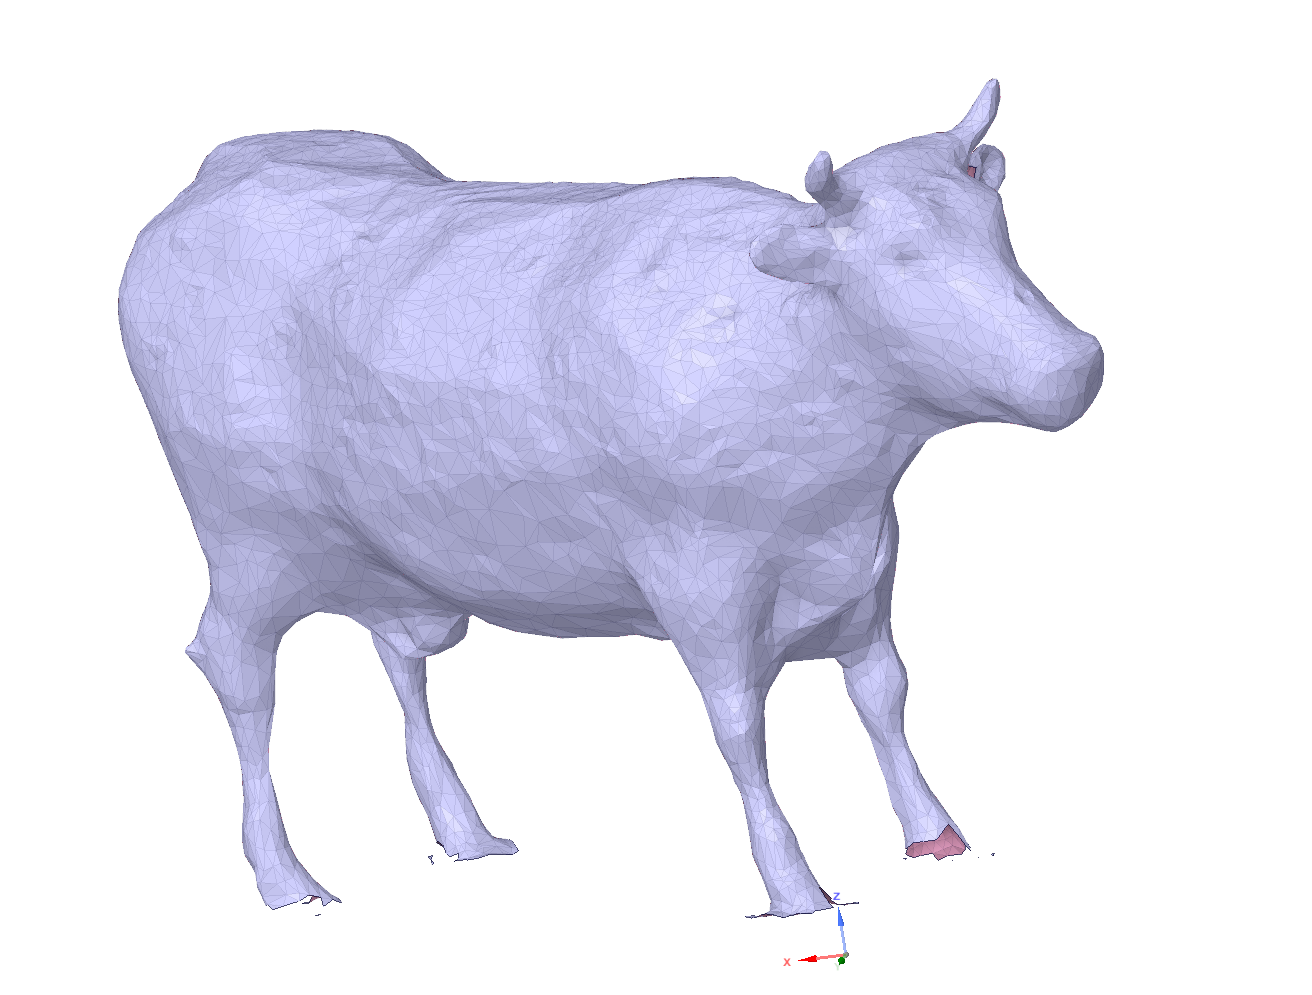
\includegraphics[width=0.5\textwidth]{cew.PNG}
    \caption{3D-Scan nach Shrinkwrap, die Euter sind zum Beispiel nicht mehr abgebildet}
    \label{fig:scangeometry}
\end{figure}

\begin{figure}[h]
    \centering
    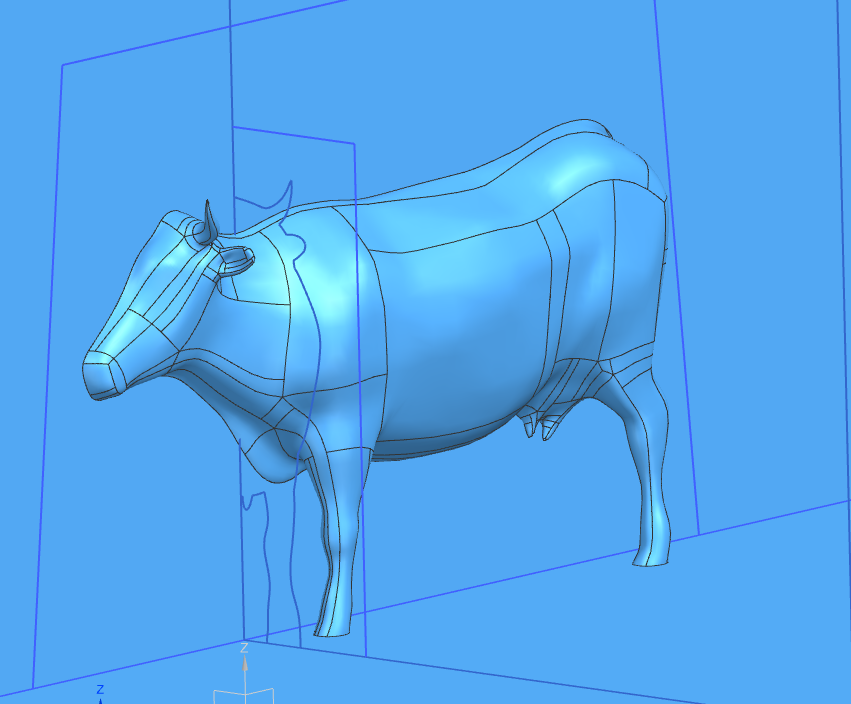
\includegraphics[width=0.5\textwidth]{nx.PNG}
    \caption{Die Originalgeometrie als prt in NX}
    \label{fig:nx}
\end{figure}

\newpage
\subsection{Material}
Es wird Luft bei 25 Grad an einem schönen Frühlingstag für die Simulation gewählt.

\subsection{Randbedingungen}
Die \( c_d \) in der Literatur sind bei einer Reynolds-Zahl zwischen \( 10^4 \) und \( 10^6 \) angegeben. Das heisst, die Luftgeschwindigkeit \( u \) wird so gewählt, dass die Reynolds-Zahl in diesen Bereich fallt.

\begin{equation}
Re = \frac{\rho u L}{\mu}
\end{equation}

Für die Simulation kann die Symmetrie der Kuh genutzt werden. Die Kuh ist als Wall no slip definiert, die Wände als Wall free slip, Inlet ist mit einer konstanten Geschwindigkeit definiert, Outlet ist als 0 Pa Druck definiert.

\subsection{Handrechnung}\label{sec:handrechnung}
Für die Handrechnung wird die Annahme aus \ref{sec:Einleitung} benutzt. Der \( c_d \)-Wert einer Sphäre kann in der \href{https://en.wikipedia.org/wiki/Drag_coefficient}{Literatur} nachgeschlagen werden und ist
$$c_d = 0.47$$

\section{Vorstudien}

Die Expression, die als Monitorpunkt benutzt wird, ist
$$ force_y@cow$$

\begin{figure}[h]
    \centering
    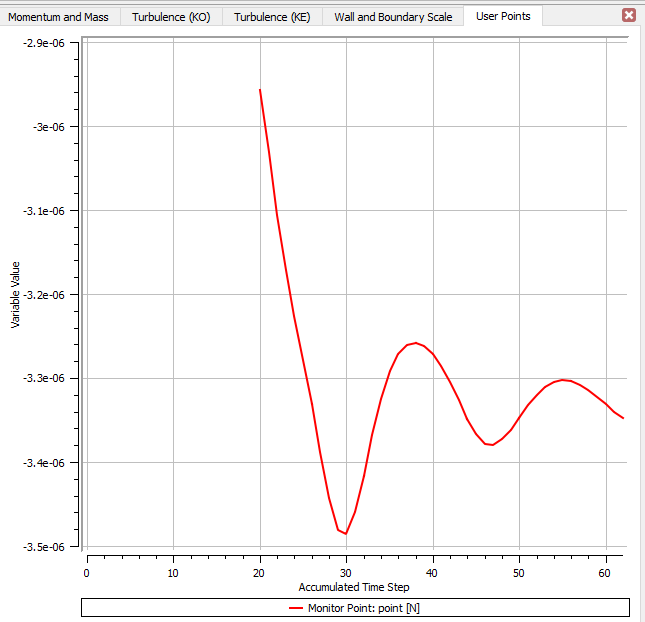
\includegraphics[width=0.5\textwidth]{force.PNG}
    \caption{Kraft auf die Fläche der Kuh}
    \label{fig:F}
\end{figure}

In Abbildung \ref{fig:F} kann gesehen werden, dass es sich leider nicht um eine turbulenz freie Strömung handelt. Um einen Wert zu bekommen, der mit dem Wert aus \ref{sec:handrechnung} verglichen werden kann, wird der Durchschnitt in den letzten Schwingungen ausgewertet.

Um die Referenzfläche \( A \) der Kuh zu erhalten, wird in NX ein Schatten der Kuh gemessen. In Abbildung \ref{fig:A} ist zu sehen, dass zum Beispiel nicht mehr berücksichtigt wird, dass eine Kuh Vorder- und Hinterbeine hat.

\begin{figure}[h]
    \centering
    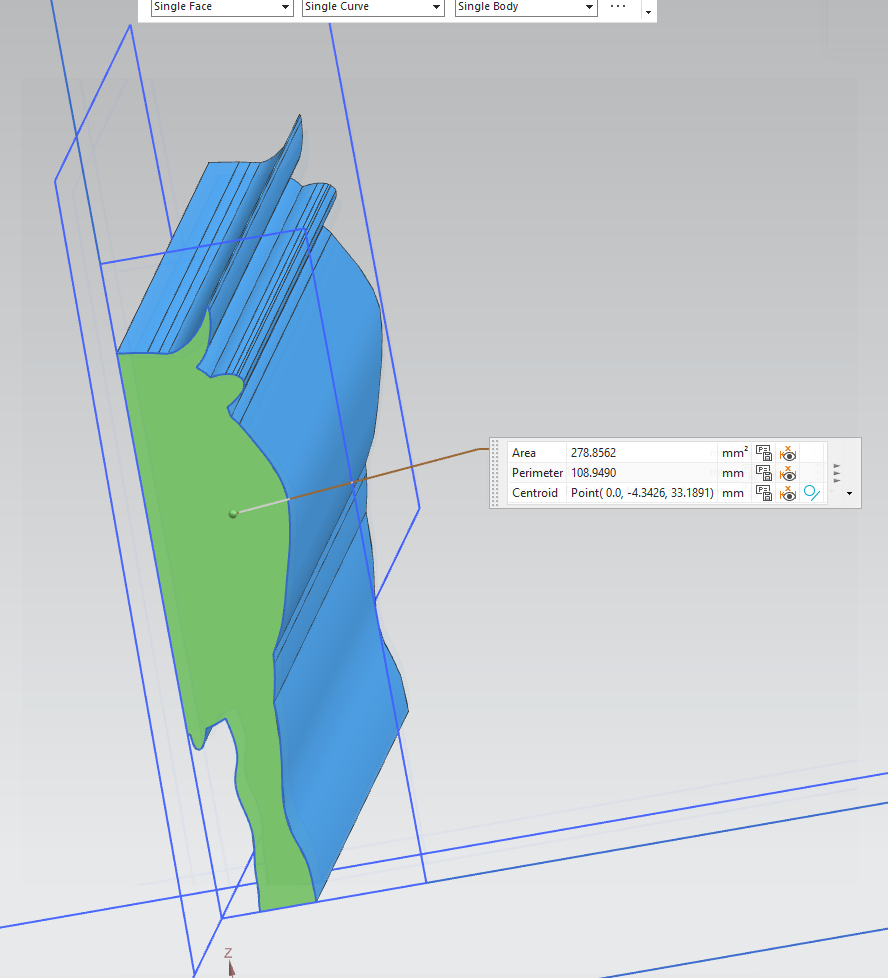
\includegraphics[width=0.5\textwidth]{surface.PNG}
    \caption{Referenzfläche der Kuh}
    \label{fig:A}
\end{figure}

\newpage

\subsection{Rechenintervalle}
Der RMS-Error in Abbildung \ref{fig:monitor1} ist nicht am konstanten Abnehmen, sondern zeigt die Eigenschaften einer Kármánschen Wirbelstrasse. Meine Vermutung ist, dass die dünnen Beine der Kuh und der massige Körper der Kuh nicht die Vorgaben der Reynolds-Zahl und keine Wirbelablösung gleichzeitig aufweisen können.

\begin{figure}[h]
    \centering
    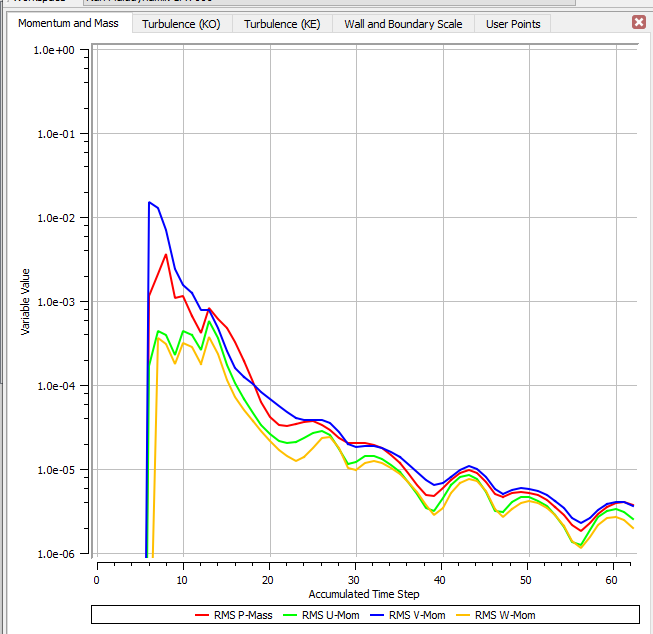
\includegraphics[width=0.5\textwidth]{rms.PNG}
    \caption{RMS-Fehler, die nicht konvergieren}
    \label{fig:monitor1}
\end{figure}

\subsection{Grösse der simulierten Luft}
Um sicherzustellen, dass die Simulation eine Kuh auf freiem Feld abbildet, muss sichergestellt werden, dass die Wände der Simulation einen vernachlässigbaren grossen Einfluss auf das Ergebnis haben. Für die Evaluation des 3D-Scans wurde eine Grösse gewählt, die dem Bauchgefühl nach ausreichend ist. Die Luft war für beide Simulationen genau gleich.

In Abbildung \ref{fig:p} kann gesehen werden, dass die Druckverteilung nicht bis an die Wände inhomogen ist, das heisst, die Wände haben tatsächlich keinen Einfluss auf die Kuh.

\begin{figure}[h]
    \centering
    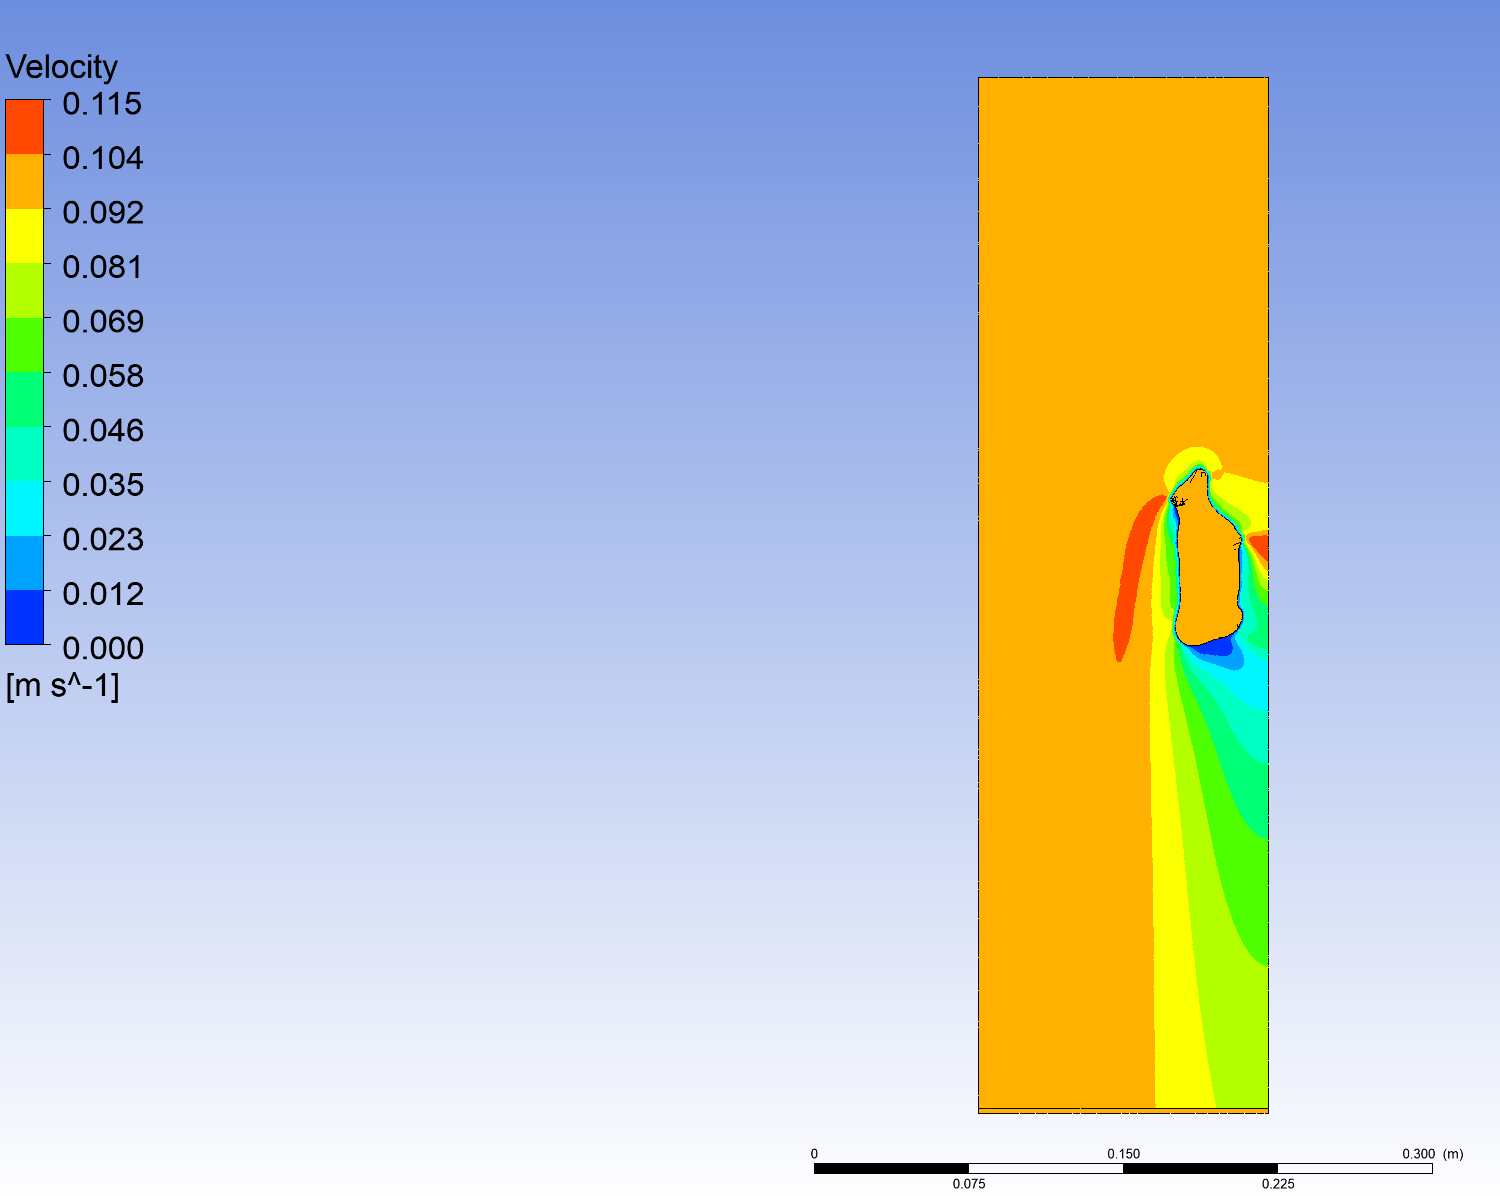
\includegraphics[width=0.5\textwidth]{Unbenannt.PNG}
    \caption{Druckverteilung über die Symmetriefläche}
    \label{fig:p}
\end{figure}

\newpage

\subsection{Netzfeinheit}
Die Netzfeinheit wird bei jedem neuen Import/Export neu definiert. Um das Modell sehr gut abzubilden, ist eine Netzfeinheit von 0.2 mm nötig. In Abbildung \ref{fig:02mesh} ist diese Feinheit zu sehen. Um mit der limitierten Hardware des VDIs ein Ergebnis erzielen zu können, musste eine Netzfeinheit von 2 mm gewählt werden. In Abbildung \ref{fig:netz} ist diese Feinheit zu sehen. Die sehr hohe Auflösung des ursprünglichen 3D-Scans stellt eine erhebliche Herausforderung für eine Simulation dar.

\begin{figure}[h]
    \centering
    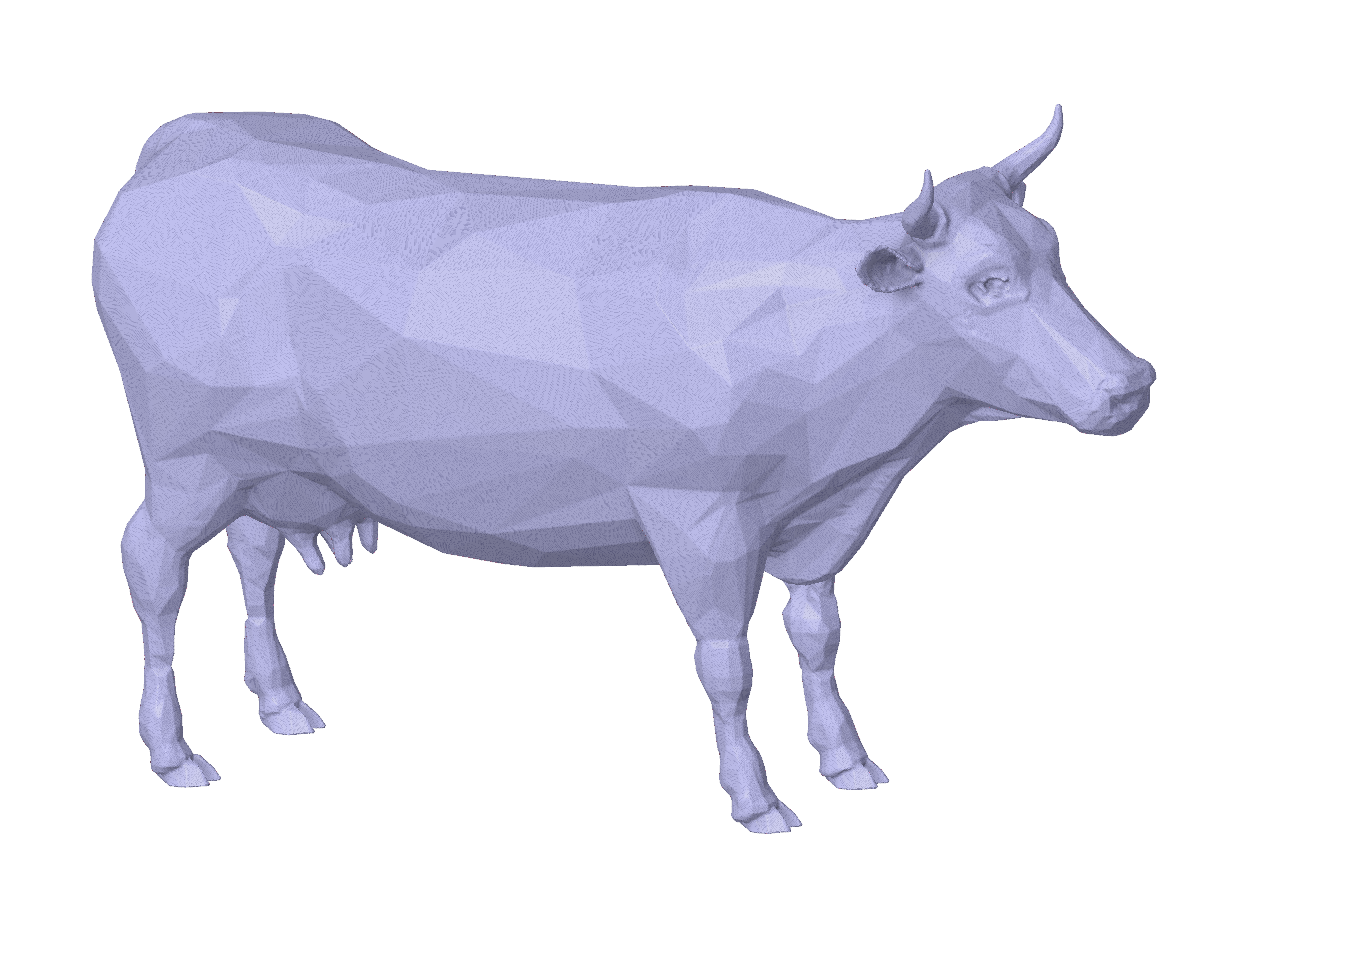
\includegraphics[width=0.5\textwidth]{cowremesh.PNG}
    \caption{Originaldatei nach Shrinkwrap, mit Netzfeinheit 0.2 mm}
    \label{fig:02mesh}
\end{figure}

\begin{figure}[h]
    \centering
    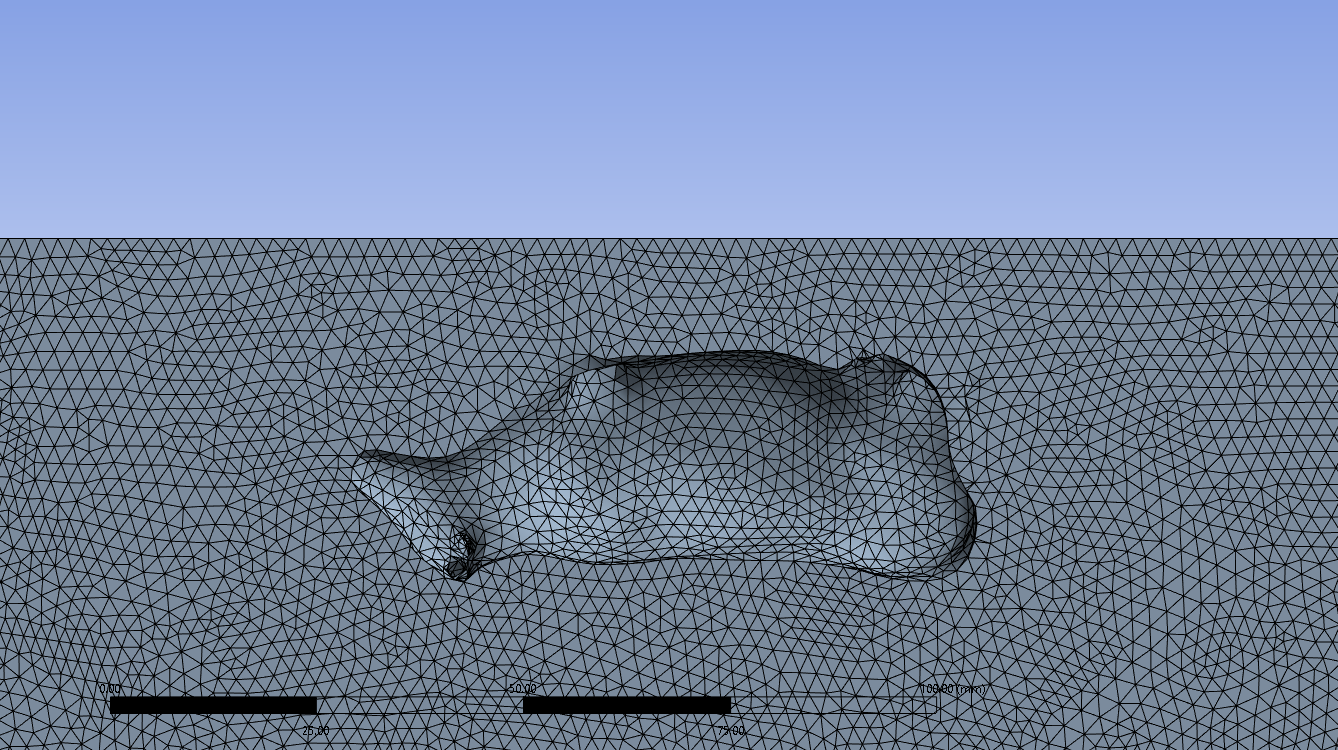
\includegraphics[width=0.5\textwidth]{nwtz.PNG}
    \caption{Simuliertes Netz, suboptimal aber konstant}
    \label{fig:netz}
\end{figure}

\newpage
\section{Ergebnisse}
Es wird ein \( c_d \) Originalwert von 0.88 und ein \( c_d \) Scanwert von 0.91 simuliert. Die Werte sind in der gleichen Grössenordnung wie die Handrechnung mit \( c_d \) Kugel und das ist alles, was der theoretische Physiker braucht.

\subsection{Plausibilität}
Die Vergleichbarkeit des Originals mit dem Scan ist schwierig, da sowohl das Original als auch der Scan durch mehrere Programme transformiert wurden. Aber es zeigt trotzdem, wie gut ein \textit{gratis} 3D-Scanner sein kann, den man immer in der Hosentasche hat.

In der Literatur \href{https://www.youtube.com/watch?v=FDG3rUx00yQ}{Youtube} wurde das gleiche Original STL für eine Berechnung benutzt und ein \( c_d \) Youtube-Wert von 0.5 ermittelt.

\section{Fazit}
Es konnte in dieser selbst gestellten Testaufgabe ein Workflow entwickelt werden, um mit einem Photogrammetrie-3D-Scanner eine CFD-Simulation durchzuführen. Die grösste Herausforderung des Workflows ist die Inkompatibilität der verschiedenen 3D-Dateitypen.

Die Simulation leidet an Turbulenzen, so konnten keine exakten Werte für den Luftwiderstand einer Kuh berechnet werden. Die beiden Simulationen und die Handrechnung sind in der gleichen Grössenordnung, somit kann in der theoretischen Physik ohne Probleme die Annahme getroffen werden, dass eine Kuh eine Kugel ist.

\end{document}
